% Options for packages loaded elsewhere
\PassOptionsToPackage{unicode}{hyperref}
\PassOptionsToPackage{hyphens}{url}
\PassOptionsToPackage{dvipsnames,svgnames,x11names}{xcolor}
%
\documentclass[
]{article}
\usepackage{amsmath,amssymb}
\usepackage{lmodern}
\usepackage{iftex}
\ifPDFTeX
  \usepackage[T1]{fontenc}
  \usepackage[utf8]{inputenc}
  \usepackage{textcomp} % provide euro and other symbols
\else % if luatex or xetex
  \usepackage{unicode-math}
  \defaultfontfeatures{Scale=MatchLowercase}
  \defaultfontfeatures[\rmfamily]{Ligatures=TeX,Scale=1}
\fi
% Use upquote if available, for straight quotes in verbatim environments
\IfFileExists{upquote.sty}{\usepackage{upquote}}{}
\IfFileExists{microtype.sty}{% use microtype if available
  \usepackage[]{microtype}
  \UseMicrotypeSet[protrusion]{basicmath} % disable protrusion for tt fonts
}{}
\makeatletter
\@ifundefined{KOMAClassName}{% if non-KOMA class
  \IfFileExists{parskip.sty}{%
    \usepackage{parskip}
  }{% else
    \setlength{\parindent}{0pt}
    \setlength{\parskip}{6pt plus 2pt minus 1pt}}
}{% if KOMA class
  \KOMAoptions{parskip=half}}
\makeatother
\usepackage{xcolor}
\usepackage{graphicx}
\makeatletter
\def\maxwidth{\ifdim\Gin@nat@width>\linewidth\linewidth\else\Gin@nat@width\fi}
\def\maxheight{\ifdim\Gin@nat@height>\textheight\textheight\else\Gin@nat@height\fi}
\makeatother
% Scale images if necessary, so that they will not overflow the page
% margins by default, and it is still possible to overwrite the defaults
% using explicit options in \includegraphics[width, height, ...]{}
\setkeys{Gin}{width=\maxwidth,height=\maxheight,keepaspectratio}
% Set default figure placement to htbp
\makeatletter
\def\fps@figure{htbp}
\makeatother
\setlength{\emergencystretch}{3em} % prevent overfull lines
\providecommand{\tightlist}{%
  \setlength{\itemsep}{0pt}\setlength{\parskip}{0pt}}
\setcounter{secnumdepth}{-\maxdimen} % remove section numbering
\newlength{\cslhangindent}
\setlength{\cslhangindent}{1.5em}
\newlength{\csllabelwidth}
\setlength{\csllabelwidth}{3em}
\newlength{\cslentryspacingunit} % times entry-spacing
\setlength{\cslentryspacingunit}{\parskip}
\newenvironment{CSLReferences}[2] % #1 hanging-ident, #2 entry spacing
 {% don't indent paragraphs
  \setlength{\parindent}{0pt}
  % turn on hanging indent if param 1 is 1
  \ifodd #1
  \let\oldpar\par
  \def\par{\hangindent=\cslhangindent\oldpar}
  \fi
  % set entry spacing
  \setlength{\parskip}{#2\cslentryspacingunit}
 }%
 {}
\usepackage{calc}
\newcommand{\CSLBlock}[1]{#1\hfill\break}
\newcommand{\CSLLeftMargin}[1]{\parbox[t]{\csllabelwidth}{#1}}
\newcommand{\CSLRightInline}[1]{\parbox[t]{\linewidth - \csllabelwidth}{#1}\break}
\newcommand{\CSLIndent}[1]{\hspace{\cslhangindent}#1}
\ifLuaTeX
\usepackage[bidi=basic]{babel}
\else
\usepackage[bidi=default]{babel}
\fi
\babelprovide[main,import]{american}
% get rid of language-specific shorthands (see #6817):
\let\LanguageShortHands\languageshorthands
\def\languageshorthands#1{}
\ifLuaTeX
  \usepackage{selnolig}  % disable illegal ligatures
\fi
\IfFileExists{bookmark.sty}{\usepackage{bookmark}}{\usepackage{hyperref}}
\IfFileExists{xurl.sty}{\usepackage{xurl}}{} % add URL line breaks if available
\urlstyle{same} % disable monospaced font for URLs
\hypersetup{
  pdftitle={MultilayerGraphs.jl: Multilayer Network Science in Julia},
  pdfauthor={Claudio Moroni, Pietro Monticone},
  pdflang={en-US},
  colorlinks=true,
  linkcolor={Maroon},
  filecolor={Maroon},
  citecolor={Blue},
  urlcolor={Blue},
  pdfcreator={LaTeX via pandoc}}

\title{MultilayerGraphs.jl: Multilayer Network Science in Julia}

%%%%%%%%%%%%%%%%%%%%%%%%%%%%%%%%%%%%%%%%%%%%%%%%%%%%%%%%%%%%%%%%%%%%%%%%
% Authors and Affiliations

\usepackage[affil-it]{authblk}
\usepackage{orcidlink}
%% \renewcommand\Authsep{, }
\setlength{\affilsep}{1em}
\author[1,2%
  *%
  ]{Claudio Moroni%
    \,\orcidlink{0000-0003-1274-6937}\,%
    }
\author[1,2%
  *%
  ]{Pietro Monticone%
    \,\orcidlink{0000-0002-2731-9623}\,%
    }

\affil[1]{University of Turin, Italy}
\affil[2]{Interdisciplinary Physics Team, Italy}
\affil[*]{These authors contributed equally.}
%%%%%%%%%%%%%%%%%%%%%%%%%%%%%%%%%%%%%%%%%%%%%%%%%%%%%%%%%%%%%%%%%%%%%%%%
\date{11 January 2023}

\begin{document}
\maketitle

\hypertarget{summary}{%
\section{Summary}\label{summary}}

\textbf{MultilayerGraphs.jl} is a Julia package for the creation,
manipulation and analysis of the structure, dynamics and functions of
multilayer graphs.

A multilayer graph consists of multiple subgraphs called \emph{layers}
which can be interconnected through
\href{https://en.wikipedia.org/wiki/Bipartite_graph}{bipartite graphs}
called \emph{interlayers} composed of the vertex sets of two different
layers and the edges between them. The vertices in each layer represent
a single set of nodes, although not all nodes have to be represented in
every layer.

Formally, a multilayer graph can be defined as a triple \(G=(V,E,L)\),
where:

\begin{itemize}
\tightlist
\item
  \(V\) is the set of vertices;
\item
  \(E\) is the set of edges, pairs of nodes \((u, v)\) representing a
  connection, relationship or interaction between the nodes \(u\) and
  \(v\);
\item
  \(L\) is a set of layers, which are subsets of \(V\) and \(E\)
  encoding the nodes and edges within each layer.
\end{itemize}

Each layer \(\ell\) in \(L\) is a tuple \((V_\ell, E_\ell)\), where
\(V_\ell\) is a subset of \(V\) that represents the vertices within that
layer, and \(E_\ell\) is a subset of \(E\) that represents the edges
within that layer.

MultilayerGraphs.jl is an integral part of the
\href{https://github.com/JuliaGraphs}{JuliaGraphs} ecosystem extending
Graphs.jl (\protect\hyperlink{ref-Graphs2021}{Fairbanks et al., 2021})
so all the methods and metrics exported by Graphs.jl work for multilayer
graphs, but due to the special nature of multilayer graphs the package
features a peculiar implementation that maps a standard integer-labelled
vertex representation to a more user-friendly framework exporting all
the objects an experienced practitioner would expect such as nodes,
vertices, layers, interlayers, etc.

MultilayerGraphs.jl features specific methods and metrics including the
global clustering coefficient, the overlay clustering coefficient, the
multilayer eigenvector centrality, the multilayer modularity and the Von
Neumann entropy.

Finally, MultilayerGraphs.jl has been integrated within the
\href{https://github.com/JuliaDynamics}{JuliaDynamics} ecosystem so that
any \texttt{Multilayer(Di)Graph} can be utilised as an argument to the
\texttt{GraphSpace} constructor in Agents.jl
(\protect\hyperlink{ref-Datseris2022}{Datseris et al., 2022}).

\begin{figure}
\centering
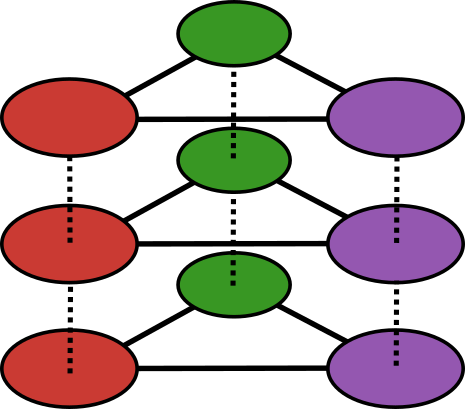
\includegraphics[width=0.25\textwidth,height=\textheight]{images/logo.png}
\caption{Logo of MultilayerGraphs.jl. \label{fig:logo}}
\end{figure}

\hypertarget{statement-of-need}{%
\section{Statement of Need}\label{statement-of-need}}

Several theoretical frameworks have been proposed to formally subsume
all instances of multilayer graphs
(\protect\hyperlink{ref-Aleta2019}{Aleta \& Moreno, 2019};
\protect\hyperlink{ref-Artime2022}{Artime et al., 2022};
\protect\hyperlink{ref-Bianconi2018}{Bianconi, 2018};
\protect\hyperlink{ref-Boccaletti2014}{Boccaletti et al., 2014};
\protect\hyperlink{ref-Cozzo2018}{Cozzo et al., 2018};
\protect\hyperlink{ref-DeDomenico2013}{M. D. Domenico et al., 2013};
\protect\hyperlink{ref-DeDomenico2022}{M. D. Domenico, 2022};
\protect\hyperlink{ref-Kivela2014}{Kivela et al., 2014};
\protect\hyperlink{ref-Lee2015}{Lee et al., 2015}).

Multilayer graphs have been adopted to model the structure and dynamics
of a wide spectrum of high-dimensional, non-linear, multi-scale,
time-dependent complex systems including physical, chemical, biological,
neuronal, socio-technical, epidemiological, ecological and economic
networks (\protect\hyperlink{ref-Aleta2022}{Aleta et al., 2022},
\protect\hyperlink{ref-Aleta2020}{2020};
\protect\hyperlink{ref-Amato2017}{Amato et al., 2017};
\protect\hyperlink{ref-deArruda2017}{Arruda et al., 2017};
\protect\hyperlink{ref-AzimiTafreshi2016}{Azimi-Tafreshi, 2016};
\protect\hyperlink{ref-Baggio2016}{Baggio et al., 2016};
\protect\hyperlink{ref-Buldu2018}{Buldú \& Porter, 2018};
\protect\hyperlink{ref-Cozzo2013}{Cozzo et al., 2013};
\protect\hyperlink{ref-DeDomenico2017}{M. D. Domenico, 2017};
\protect\hyperlink{ref-DeDomenico2016}{M. D. Domenico et al., 2016};
\protect\hyperlink{ref-Estrada2014}{Estrada \& Gómez-Gardeñes, 2014};
\protect\hyperlink{ref-Gosak2018}{Gosak et al., 2018};
\protect\hyperlink{ref-Granell2013}{Granell et al., 2013};
\protect\hyperlink{ref-Lim2019}{Lim et al., 2019};
\protect\hyperlink{ref-Mangioni2020}{Mangioni et al., 2020};
\protect\hyperlink{ref-Massaro2014}{Massaro \& Bagnoli, 2014};
\protect\hyperlink{ref-Pilosof2017}{Pilosof et al., 2017};
\protect\hyperlink{ref-SorianoPaos2018}{Soriano-Paños et al., 2018};
\protect\hyperlink{ref-Timteo2018}{Timóteo et al., 2018}).

At the best of our knowledge there are currently no software packages
dedicated to the creation, manipulation and analysis of multilayer
graphs implemented in the \href{https://julialang.org}{Julia language}
(\protect\hyperlink{ref-Bezanson2017}{Bezanson et al., 2017}) apart from
MultilayerGraphs.jl itself
(\protect\hyperlink{ref-Moroni_Monticone_MultilayerGraphs_2022}{Moroni
\& Monticone, 2022}).

\begin{figure}
\centering
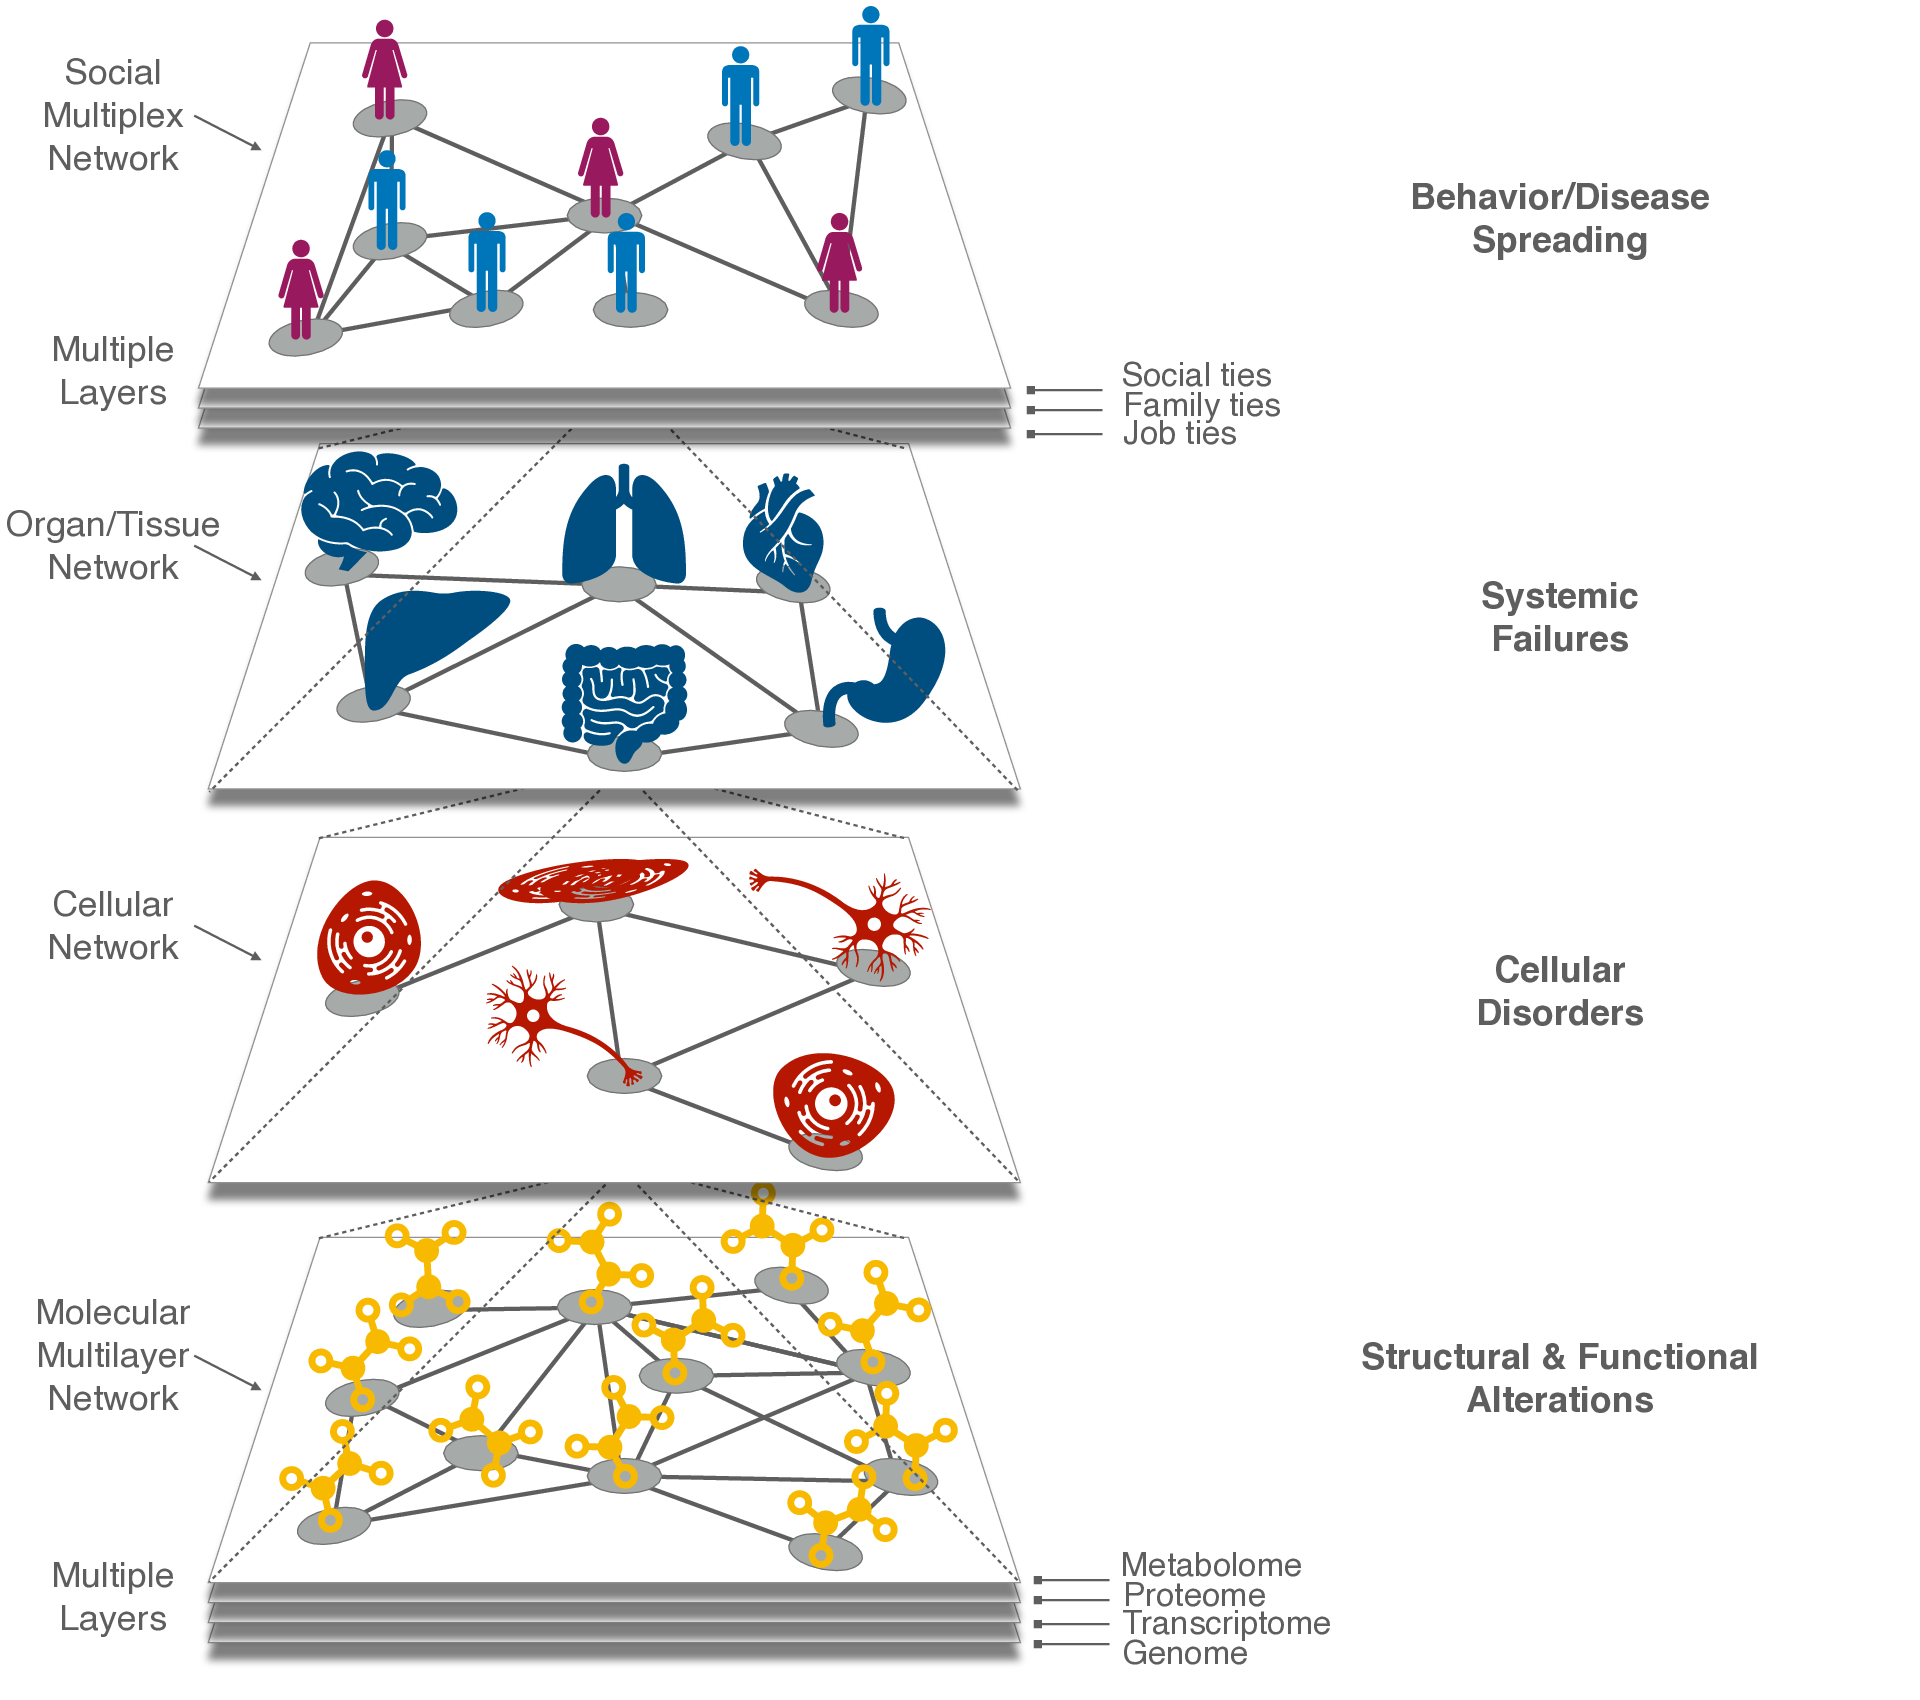
\includegraphics[width=1\textwidth,height=\textheight]{images/application_biology.png}
\caption{Diagram illustrating a multi-scale multilayer graph applied to
model social systems from the molecular to the population level
(\protect\hyperlink{ref-DeDomenicoIllustrated2022}{De Domenico, 2022}).
\label{fig:application-biology}}
\end{figure}

\hypertarget{main-features}{%
\section{Main Features}\label{main-features}}

The two main data structures are collections of layers connected through
interlayers called \texttt{MultilayerGraph} and
\texttt{MultilayerDiGraph}.

The \textbf{vertices} of a multilayer graph are representations of one
set of distinct objects called \texttt{Node}s. Each layer may represent
all the node set or just a subset of it. The vertices of
\texttt{Multilayer(Di)Graph} are implemented via the
\texttt{MultilayerVertex} custom type. Each \texttt{MultilayerVertex}
encodes information about the node it represents, the layer it belongs
to and its metadata.

Both the \textbf{intra-layer} and \textbf{inter-layer edges} are
embedded in the \texttt{MultilayerEdge} struct, whose arguments are the
two connected multilayer vertices, the edge weight and its metadata.
It's important to highlight that \texttt{Multilayer(Di)Graph}s are
weighted and able to store metadata by default (i.e.~they have been
assigned the \texttt{IsWeighted} and \texttt{IsMeta} traits from
\href{https://github.com/mauro3/SimpleTraits.jl}{SimpleTraits.jl}).

The \textbf{layers} are implemented via the \texttt{Layer} struct
composed of an underlying graph and a mapping from its integer-labelled
vertices to the collection of \texttt{MultilayerVertex}s the layer
represents. \textbf{Interlayers} are similarly implemented via the
\texttt{Interlayer} mutable struct, and they are generally constructed
by providing the two connected layers, the (multilayer) edge list
between them and a graph. This usage of underlying graphs allows for an
easier debugging procedure during construction and a more intuitive
analysis afterwards allowing the package to leverage all the features of
the JuliaGraphs ecosystem so that it can be effectively considered as a
real proving ground of its internal consistency.

The \texttt{Multilayer(Di)Graph} structs are weighted and endowed with
the functionality to store both vertex-level and edge-level metadata by
default so that at any moment the user may add or remove a
\texttt{Layer} or specify an \texttt{Interlayer} and since different
layers and interlayers could be better represented by graphs that are
weighted or unweighted and with or without metadata, it was crucial for
us to provide the most general and adaptable structure. A
\texttt{Multilayer(Di)Graph} is instantiated by providing the ordered
list of layers and the list of interlayers to the constructor. The
latter are automatically specified, so there is no need to instantiate
all of them.

Alternatively, it is possible to construct a
\texttt{Multilayer(Di)Graph} making use of a graph generator-like
signature allowing the user to set the degree distribution or the degree
sequence and employs graph realisation methods such as the Havel-Hakimi
algorithm for undirected graphs
(\protect\hyperlink{ref-Hakimi1962}{Hakimi, 1962}) and the Kleitman-Wang
algorithm for directed ones
(\protect\hyperlink{ref-Kleitman1973}{Kleitman \& Wang, 1973}).

\texttt{Multilayer(Di)Graph}s structure may be represented via dedicated
\texttt{WeightTensor}, \texttt{MetadataTensor} and
\texttt{SupraWeightMatrix} structs, all of which support indexing with
\texttt{MultilayerVertex}s. Once a \texttt{Multilayer(Di)Graph} has been
instantiated, its layers and interlayers can be accessed as their
properties.

For a more comprehensive exploration of the package features and
functionalities we strongly recommend consulting the package
\href{https://github.com/JuliaGraphs/MultilayerGraphs.jl/blob/main/README.md}{README}
and \href{https://juliagraphs.org/MultilayerGraphs.jl}{documentation}.

\hypertarget{installation-and-usage}{%
\section{Installation and Usage}\label{installation-and-usage}}

We invite the user to read the documented
\href{https://github.com/JuliaGraphs/MultilayerGraphs.jl/tree/main/example/example.md}{example}
and run the associated
\href{https://github.com/JuliaGraphs/MultilayerGraphs.jl/blob/main/example/example.jl}{script}
we have designed to synthetically illustrate:

\begin{itemize}
\tightlist
\item
  how to \textbf{install} the package;
\item
  how to define \textbf{layers} and \textbf{interlayers} with a variety
  of constructors and underlying graphs;
\item
  how to construct a \textbf{directed multilayer graph} with those
  layers and interlayers;
\item
  how to add \textbf{nodes}, \textbf{vertices} and \textbf{edges} to the
  multilayer graph;
\item
  how to compute some multilayer \textbf{metrics} as defined in M. D.
  Domenico et al. (\protect\hyperlink{ref-DeDomenico2013}{2013}).
\end{itemize}

\hypertarget{related-packages}{%
\section{Related Packages}\label{related-packages}}

\hypertarget{r}{%
\subsection{R}\label{r}}

Here is a list of related software packages implemented in the
\href{https://www.r-project.org}{R language}:

\begin{itemize}
\tightlist
\item
  \href{https://github.com/manlius/muxViz}{\texttt{muxViz}} implements
  functions to perform multilayer correlation analysis, multilayer
  centrality analysis, multilayer community structure detection,
  multilayer structural reducibility, multilayer motifs analysis and
  utilities to statically and dynamically visualise multilayer graphs
  (\protect\hyperlink{ref-DeDomenico2014}{D. Domenico et al., 2014});
\item
  \href{https://github.com/cran/multinet}{\texttt{multinet}} implements
  functions to import, export, create and manipulate multilayer graphs,
  several state-of-the-art multiplex graph analysis algorithms for
  centrality measures, layer comparison, community detection and
  visualization (\protect\hyperlink{ref-Magnani2021}{Magnani et al.,
  2021});
\item
  \href{https://github.com/frankkramer-lab/mully}{\texttt{mully}}
  implements functions to import, export, create, manipulate and merge
  multilayer graphs and utilities to visualise multilayer graphs in 2D
  and 3D (\protect\hyperlink{ref-Hammoud2018}{Hammoud \& Kramer, 2018});
\item
  \href{https://github.com/neylsoncrepalde/multinets}{\texttt{multinets}}
  implements functions to import, export, create, manipulate multilayer
  graphs and utilities to visualise multilayer graphs
  (\protect\hyperlink{ref-Lazega2008}{Lazega et al., 2008}).
\end{itemize}

\hypertarget{python}{%
\subsection{Python}\label{python}}

Here is a list of related software packages implemented in the
\href{https://www.python.org}{Python language}:

\begin{itemize}
\tightlist
\item
  \href{https://github.com/nkoub/multinetx}{\texttt{MultiNetX}}
  implements methods to create undirected networks with weighted or
  unweighted links, to analyse the spectral properties of adjacency or
  Laplacian matrices and to visualise multilayer graphs and dynamical
  processes by coloring the nodes and links accordingly;
\item
  \href{https://github.com/bolozna/Multilayer-networks-library}{\texttt{PyMNet}}
  implements data structures for multilayer graphs and multiplex graphs,
  methods to import, export, create, manipulate multilayer graphs and
  for the rule-based generation and lazy-evaluation of coupling edges
  and utilities to visualise multilayer graphs
  (\protect\hyperlink{ref-Kivela2014}{Kivela et al., 2014}).
\end{itemize}

\hypertarget{acknowledgements}{%
\section{Acknowledgements}\label{acknowledgements}}

This open-source research software project received no financial
support.

\hypertarget{references}{%
\section*{References}\label{references}}
\addcontentsline{toc}{section}{References}

\hypertarget{refs}{}
\begin{CSLReferences}{1}{0}
\leavevmode\vadjust pre{\hypertarget{ref-Aleta2022}{}}%
Aleta, A., Martı́n-Corral, D., Bakker, M. A., Piontti, A. P. y, Ajelli,
M., Litvinova, M., Chinazzi, M., Dean, N. E., Halloran, M. E., Longini,
I. M., Pentland, A., Vespignani, A., Moreno, Y., \& Moro, E. (2022).
Quantifying the importance and location of {SARS}-{CoV}-2 transmission
events in large metropolitan areas. \emph{Proceedings of the National
Academy of Sciences}, \emph{119}(26).
\url{https://doi.org/10.1073/pnas.2112182119}

\leavevmode\vadjust pre{\hypertarget{ref-Aleta2020}{}}%
Aleta, A., Martı́n-Corral, D., Piontti, A. P. y, Ajelli, M., Litvinova,
M., Chinazzi, M., Dean, N. E., Halloran, M. E., Jr, I. M. L., Merler,
S., Pentland, A., Vespignani, A., Moro, E., \& Moreno, Y. (2020).
Modelling the impact of testing, contact tracing and household
quarantine on second waves of {COVID}-19. \emph{Nature Human Behaviour},
\emph{4}(9), 964--971. \url{https://doi.org/10.1038/s41562-020-0931-9}

\leavevmode\vadjust pre{\hypertarget{ref-Aleta2019}{}}%
Aleta, A., \& Moreno, Y. (2019). Multilayer networks in a nutshell.
\emph{Annual Review of Condensed Matter Physics}, \emph{10}(1), 45--62.
\url{https://doi.org/10.1146/annurev-conmatphys-031218-013259}

\leavevmode\vadjust pre{\hypertarget{ref-Amato2017}{}}%
Amato, R., Dı́az-Guilera, A., \& Kleineberg, K.-K. (2017). Interplay
between social influence and competitive strategical games in multiplex
networks. \emph{Scientific Reports}, \emph{7}(1).
\url{https://doi.org/10.1038/s41598-017-06933-2}

\leavevmode\vadjust pre{\hypertarget{ref-deArruda2017}{}}%
Arruda, G. F. de, Cozzo, E., Peixoto, T. P., Rodrigues, F. A., \&
Moreno, Y. (2017). Disease localization in multilayer networks.
\emph{Physical Review X}, \emph{7}(1).
\url{https://doi.org/10.1103/physrevx.7.011014}

\leavevmode\vadjust pre{\hypertarget{ref-Artime2022}{}}%
Artime, O., Benigni, B., Bertagnolli, G., dAndrea, V., Gallotti, R.,
Ghavasieh, A., Raimondo, S., \& Domenico, M. D. (2022). \emph{Multilayer
network science}. Cambridge University Press.
\url{https://doi.org/10.1017/9781009085809}

\leavevmode\vadjust pre{\hypertarget{ref-AzimiTafreshi2016}{}}%
Azimi-Tafreshi, N. (2016). Cooperative epidemics on multiplex networks.
\emph{Physical Review E}, \emph{93}(4).
\url{https://doi.org/10.1103/physreve.93.042303}

\leavevmode\vadjust pre{\hypertarget{ref-Baggio2016}{}}%
Baggio, J. A., BurnSilver, S. B., Arenas, A., Magdanz, J. S., Kofinas,
G. P., \& Domenico, M. D. (2016). Multiplex social ecological network
analysis reveals how social changes affect community robustness more
than resource depletion. \emph{Proceedings of the National Academy of
Sciences}, \emph{113}(48), 13708--13713.
\url{https://doi.org/10.1073/pnas.1604401113}

\leavevmode\vadjust pre{\hypertarget{ref-Bezanson2017}{}}%
Bezanson, J., Edelman, A., Karpinski, S., \& Shah, V. B. (2017). Julia:
A fresh approach to numerical computing. \emph{{SIAM} Review},
\emph{59}(1), 65--98. \url{https://doi.org/10.1137/141000671}

\leavevmode\vadjust pre{\hypertarget{ref-Bianconi2018}{}}%
Bianconi, G. (2018). \emph{Multilayer networks}. Oxford University
Press. \url{https://doi.org/10.1093/oso/9780198753919.001.0001}

\leavevmode\vadjust pre{\hypertarget{ref-Boccaletti2014}{}}%
Boccaletti, S., Bianconi, G., Criado, R., Genio, C. I. del,
Gómez-Gardeñes, J., Romance, M., Sendiña-Nadal, I., Wang, Z., \& Zanin,
M. (2014). The structure and dynamics of multilayer networks.
\emph{Physics Reports}, \emph{544}(1), 1--122.
\url{https://doi.org/10.1016/j.physrep.2014.07.001}

\leavevmode\vadjust pre{\hypertarget{ref-Buldu2018}{}}%
Buldú, J. M., \& Porter, M. A. (2018). Frequency-based brain networks:
From a multiplex framework to a full multilayer description.
\emph{Network Neuroscience}, \emph{2}(4), 418--441.
\url{https://doi.org/10.1162/netn_a_00033}

\leavevmode\vadjust pre{\hypertarget{ref-Cozzo2018}{}}%
Cozzo, E., Arruda, G. F. de, Rodrigues, F. A., \& Moreno, Y. (2018).
\emph{Multiplex networks}. Springer International Publishing.
\url{https://doi.org/10.1007/978-3-319-92255-3}

\leavevmode\vadjust pre{\hypertarget{ref-Cozzo2013}{}}%
Cozzo, E., Baños, R. A., Meloni, S., \& Moreno, Y. (2013). Contact-based
social contagion in multiplex networks. \emph{Physical Review E},
\emph{88}(5). \url{https://doi.org/10.1103/physreve.88.050801}

\leavevmode\vadjust pre{\hypertarget{ref-Datseris2022}{}}%
Datseris, G., Vahdati, A. R., \& DuBois, T. C. (2022). Agents.jl: A
performant and feature-full agent-based modeling software of minimal
code complexity. \emph{{SIMULATION}}, 003754972110688.
\url{https://doi.org/10.1177/00375497211068820}

\leavevmode\vadjust pre{\hypertarget{ref-DeDomenicoIllustrated2022}{}}%
De Domenico, M. (2022). \emph{Multilayer networks illustrated}.
\url{https://doi.org/10.17605/OSF.IO/GY53K}

\leavevmode\vadjust pre{\hypertarget{ref-DeDomenico2014}{}}%
Domenico, D., Porter, \& Arenas. (2014). {MuxViz}: A tool for multilayer
analysis and visualization of networks. \emph{Journal of Complex
Networks}, \emph{3}(2), 159--176.
\url{https://doi.org/10.1093/comnet/cnu038}

\leavevmode\vadjust pre{\hypertarget{ref-DeDomenico2017}{}}%
Domenico, M. D. (2017). Multilayer modeling and analysis of human brain
networks. \emph{{GigaScience}}, \emph{6}(5).
\url{https://doi.org/10.1093/gigascience/gix004}

\leavevmode\vadjust pre{\hypertarget{ref-DeDomenico2022}{}}%
Domenico, M. D. (2022). \emph{Multilayer networks: Analysis and
visualization}. Springer International Publishing.
\url{https://doi.org/10.1007/978-3-030-75718-2}

\leavevmode\vadjust pre{\hypertarget{ref-DeDomenico2016}{}}%
Domenico, M. D., Granell, C., Porter, M. A., \& Arenas, A. (2016). The
physics of spreading processes in multilayer~networks. \emph{Nature
Physics}, \emph{12}(10), 901--906.
\url{https://doi.org/10.1038/nphys3865}

\leavevmode\vadjust pre{\hypertarget{ref-DeDomenico2013}{}}%
Domenico, M. D., Solé-Ribalta, A., Cozzo, E., Kivelä, M., Moreno, Y.,
Porter, M. A., Gómez, S., \& Arenas, A. (2013). Mathematical formulation
of multilayer networks. \emph{Physical Review X}, \emph{3}(4).
\url{https://doi.org/10.1103/physrevx.3.041022}

\leavevmode\vadjust pre{\hypertarget{ref-Estrada2014}{}}%
Estrada, E., \& Gómez-Gardeñes, J. (2014). Communicability reveals a
transition to coordinated behavior in multiplex networks. \emph{Physical
Review E}, \emph{89}(4).
\url{https://doi.org/10.1103/physreve.89.042819}

\leavevmode\vadjust pre{\hypertarget{ref-Graphs2021}{}}%
Fairbanks, J., Besançon, M., Simon, S., Hoffiman, J., Eubank, N., \&
Karpinski, S. (2021). \emph{JuliaGraphs/graphs.jl: An optimized graphs
package for the julia programming language}.
\url{https://github.com/JuliaGraphs/Graphs.jl/}

\leavevmode\vadjust pre{\hypertarget{ref-Gosak2018}{}}%
Gosak, M., Markovič, R., Dolenšek, J., Rupnik, M. S., Marhl, M., Stožer,
A., \& Perc, M. (2018). Network science of biological systems at
different scales: A review. \emph{Physics of Life Reviews}, \emph{24},
118--135. \url{https://doi.org/10.1016/j.plrev.2017.11.003}

\leavevmode\vadjust pre{\hypertarget{ref-Granell2013}{}}%
Granell, C., Gómez, S., \& Arenas, A. (2013). Dynamical interplay
between awareness and epidemic spreading in multiplex networks.
\emph{Physical Review Letters}, \emph{111}(12).
\url{https://doi.org/10.1103/physrevlett.111.128701}

\leavevmode\vadjust pre{\hypertarget{ref-Hakimi1962}{}}%
Hakimi, S. L. (1962). On realizability of a set of integers as degrees
of the vertices of a linear graph. i. \emph{Journal of the Society for
Industrial and Applied Mathematics}, \emph{10}(3), 496--506.
\url{https://doi.org/10.1137/0110037}

\leavevmode\vadjust pre{\hypertarget{ref-Hammoud2018}{}}%
Hammoud, Z., \& Kramer, F. (2018). Mully: An r package to create, modify
and visualize multilayered graphs. \emph{Genes}, \emph{9}(11), 519.
\url{https://doi.org/10.3390/genes9110519}

\leavevmode\vadjust pre{\hypertarget{ref-Kivela2014}{}}%
Kivela, M., Arenas, A., Barthelemy, M., Gleeson, J. P., Moreno, Y., \&
Porter, M. A. (2014). Multilayer networks. \emph{Journal of Complex
Networks}, \emph{2}(3), 203--271.
\url{https://doi.org/10.1093/comnet/cnu016}

\leavevmode\vadjust pre{\hypertarget{ref-Kleitman1973}{}}%
Kleitman, D. J., \& Wang, D. L. (1973). Algorithms for constructing
graphs and digraphs with given valences and factors. \emph{Discrete
Mathematics}, \emph{6}(1), 79--88.
\url{https://doi.org/10.1016/0012-365x(73)90037-x}

\leavevmode\vadjust pre{\hypertarget{ref-Lazega2008}{}}%
Lazega, E., Jourda, M.-T., Mounier, L., \& Stofer, R. (2008). Catching
up with big fish in the big pond? Multi-level network analysis through
linked design. \emph{Social Networks}, \emph{30}(2), 159--176.
\url{https://doi.org/10.1016/j.socnet.2008.02.001}

\leavevmode\vadjust pre{\hypertarget{ref-Lee2015}{}}%
Lee, K.-M., Min, B., \& Goh, K.-I. (2015). Towards real-world
complexity: An introduction to multiplex networks. \emph{The European
Physical Journal B}, \emph{88}(2).
\url{https://doi.org/10.1140/epjb/e2015-50742-1}

\leavevmode\vadjust pre{\hypertarget{ref-Lim2019}{}}%
Lim, S., Radicchi, F., Heuvel, M. P. van den, \& Sporns, O. (2019).
Discordant attributes of structural and functional brain connectivity in
a two-layer multiplex network. \emph{Scientific Reports}, \emph{9}(1).
\url{https://doi.org/10.1038/s41598-019-39243-w}

\leavevmode\vadjust pre{\hypertarget{ref-Magnani2021}{}}%
Magnani, M., Rossi, L., \& Vega, D. (2021). Analysis of multiplex social
networks with r. \emph{Journal of Statistical Software}, \emph{98}(8).
\url{https://doi.org/10.18637/jss.v098.i08}

\leavevmode\vadjust pre{\hypertarget{ref-Mangioni2020}{}}%
Mangioni, G., Jurman, G., \& Domenico, M. D. (2020). Multilayer flows in
molecular networks identify biological modules in the human proteome.
\emph{{IEEE} Transactions on Network Science and Engineering},
\emph{7}(1), 411--420. \url{https://doi.org/10.1109/tnse.2018.2871726}

\leavevmode\vadjust pre{\hypertarget{ref-Massaro2014}{}}%
Massaro, E., \& Bagnoli, F. (2014). Epidemic spreading and risk
perception in multiplex networks: A self-organized percolation method.
\emph{Physical Review E}, \emph{90}(5).
\url{https://doi.org/10.1103/physreve.90.052817}

\leavevmode\vadjust pre{\hypertarget{ref-Moroni_Monticone_MultilayerGraphs_2022}{}}%
Moroni, C., \& Monticone, P. (2022). \emph{MultilayerGraphs.jl: A julia
package for the creation, manipulation and analysis of the structure,
dynamics and functions of multilayer graphs}. University of Turin
(UniTO); Interdisciplinary Physics Team (InPhyT).
\url{https://doi.org/10.5281/zenodo.7009172}

\leavevmode\vadjust pre{\hypertarget{ref-Pilosof2017}{}}%
Pilosof, S., Porter, M. A., Pascual, M., \& Kéfi, S. (2017). The
multilayer nature of ecological networks. \emph{Nature Ecology
{\&}Amp\(\mathsemicolon\) Evolution}, \emph{1}(4).
\url{https://doi.org/10.1038/s41559-017-0101}

\leavevmode\vadjust pre{\hypertarget{ref-SorianoPaos2018}{}}%
Soriano-Paños, D., Lotero, L., Arenas, A., \& Gómez-Gardeñes, J. (2018).
Spreading processes in multiplex metapopulations containing different
mobility networks. \emph{Physical Review X}, \emph{8}(3).
\url{https://doi.org/10.1103/physrevx.8.031039}

\leavevmode\vadjust pre{\hypertarget{ref-Timteo2018}{}}%
Timóteo, S., Correia, M., Rodrı́guez-Echeverrı́a, S., Freitas, H., \&
Heleno, R. (2018). Multilayer networks reveal the spatial structure of
seed-dispersal interactions across the great rift landscapes.
\emph{Nature Communications}, \emph{9}(1).
\url{https://doi.org/10.1038/s41467-017-02658-y}

\end{CSLReferences}

\end{document}
